\documentclass[tikz,border=2pt]{standalone}
\usepackage{amsmath}
\usepackage{amssymb}
\usepackage{xcolor}

\definecolor{journalink}{HTML}{1F1C18}
\definecolor{journalmuted}{HTML}{8A7F72}
\definecolor{journalaccent}{HTML}{9C2D2D}

\begin{document}
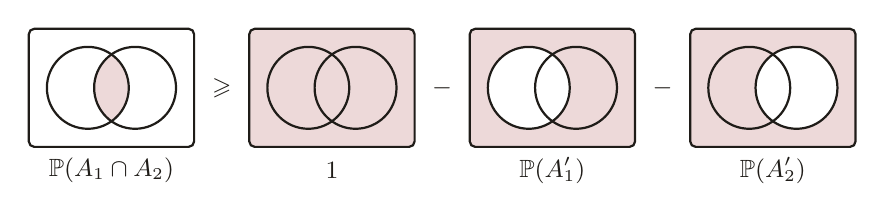
\begin{tikzpicture}[
  x=1cm,
  y=1cm,
  every node/.style={font=\small}
]
  \def\panelbox{(-0.75,-0.75) rectangle (1.35,0.75)}
  \def\circleA{(0,0) circle (0.52)}
  \def\circleB{(0.6,0) circle (0.52)}

  % Panel 1: P(A1 cap A2)
  \begin{scope}[shift={(0,0)}]
    \begin{scope}
      \clip \circleA;
      \path[fill=journalaccent, fill opacity=0.18] \circleB;
    \end{scope}
    \draw[journalink, line width=0.8pt, rounded corners=2pt] \panelbox;
    \draw[journalink, line width=0.8pt] \circleA;
    \draw[journalink, line width=0.8pt] \circleB;
    \node[journalink] at (0.3,-1.05) {$\mathbb{P}(A_1\cap A_2)$};
    \node[journalink] at (1.7,0) {$\geqslant$};
  \end{scope}

  % Panel 2: 1 (whole box shaded)
  \begin{scope}[shift={(2.8,0)}]
    \path[fill=journalaccent, fill opacity=0.18, rounded corners=2pt] \panelbox;
    \draw[journalink, line width=0.8pt, rounded corners=2pt] \panelbox;
    \draw[journalink, line width=0.8pt] \circleA;
    \draw[journalink, line width=0.8pt] \circleB;
    \node[journalink] at (0.3,-1.05) {$1$};
    \node[journalink] at (1.7,0) {$-$};
  \end{scope}

  % Panel 3: P(A1') (box minus A1 shaded)
  \begin{scope}[shift={(5.6,0)}]
    \begin{scope}[even odd rule]
      \clip \circleA (-0.75,-0.75) rectangle (1.35,0.75);
      \path[fill=journalaccent, fill opacity=0.18, rounded corners=2pt] \panelbox;
    \end{scope}
    \draw[journalink, line width=0.8pt, rounded corners=2pt] \panelbox;
    \draw[journalink, line width=0.8pt] \circleA;
    \draw[journalink, line width=0.8pt] \circleB;
    \node[journalink] at (0.3,-1.05) {$\mathbb{P}(A_1^{\prime})$};
    \node[journalink] at (1.7,0) {$-$};
  \end{scope}

  % Panel 4: P(A2') (box minus A2 shaded)
  \begin{scope}[shift={(8.4,0)}]
    \begin{scope}[even odd rule]
      \clip \circleB (-0.75,-0.75) rectangle (1.35,0.75);
      \path[fill=journalaccent, fill opacity=0.18, rounded corners=2pt] \panelbox;
    \end{scope}
    \draw[journalink, line width=0.8pt, rounded corners=2pt] \panelbox;
    \draw[journalink, line width=0.8pt] \circleA;
    \draw[journalink, line width=0.8pt] \circleB;
    \node[journalink] at (0.3,-1.05) {$\mathbb{P}(A_2^{\prime})$};
  \end{scope}
\end{tikzpicture}
\end{document}
